\documentclass[zihao=false,fontset=windows]{ctexart}
% ctexart 不接受任意 pt 选项。正文改 {10pt}，方括号里是行距。
\usepackage{scrextend}
\changefontsizes[12pt]{10pt}

\usepackage[a4paper,left=2.35cm,right=2.35cm,top=1.7cm,bottom=1.9cm]{geometry}
\usepackage{xcolor}
\usepackage{graphicx}
\usepackage{amsmath,amssymb}
\usepackage{enumitem}
\usepackage{tabularx}
\usepackage{colortbl}
\usepackage{multirow}
\usepackage{listings}
\usepackage{hyperref}
\usepackage[most]{tcolorbox}

\definecolor{feishuText}{RGB}{31,35,41}
\definecolor{feishuBlue}{RGB}{36,91,219}
\definecolor{feishuRed}{RGB}{216,57,49}
\definecolor{feishuGreen}{RGB}{46,161,33}
\definecolor{feishuPurple}{RGB}{100,37,208}
\definecolor{feishuGray}{RGB}{100,106,115}
\definecolor{feishuGray2}{RGB}{143,149,158}
\definecolor{feishuPinkBg}{RGB}{251,191,188}
\definecolor{quoteBar}{RGB}{51,112,255}
\definecolor{codebg}{RGB}{245,246,247}
\definecolor{codeborder}{RGB}{222,224,227}
\definecolor{inlinebg}{RGB}{242,243,245}
\definecolor{callRed}{RGB}{253,226,226}
\definecolor{callOrange}{RGB}{255,245,235}
\definecolor{callYellow}{RGB}{254,255,240}
\definecolor{callGreen}{RGB}{240,251,239}
\definecolor{callBlue}{RGB}{240,244,255}
\definecolor{callIce}{RGB}{225,234,255}
\definecolor{callRedSoft}{RGB}{254,241,241}
\definecolor{callSun}{RGB}{255,255,204}
\definecolor{hlYellow}{RGB}{255,246,122}
\definecolor{hlGreen}{RGB}{183,237,177}
\definecolor{hlBlue}{RGB}{186,206,253}
\definecolor{hlPurple}{RGB}{205,178,250}
\definecolor{hlOrange}{RGB}{254,212,164}
\definecolor{tableHead}{RGB}{242,243,245}
\definecolor{tableRule}{RGB}{222,224,227}
\definecolor{codeText}{RGB}{31,35,41}
\definecolor{codeKeyword}{RGB}{0,0,255}
\definecolor{codeComment}{RGB}{0,128,0}
\definecolor{codeString}{RGB}{163,21,21}

\setmainfont{Times New Roman}
\setCJKmainfont{Microsoft YaHei}[AutoFakeBold=2.2]
\setCJKsansfont{Microsoft YaHei}[AutoFakeBold=2.2]
\setCJKmonofont{Microsoft YaHei}[AutoFakeBold=2.2]
\setmonofont{Consolas}
\newfontfamily\emojifont{Segoe UI Emoji}

\hypersetup{
  colorlinks=true,
  urlcolor=feishuBlue,
  linkcolor=feishuBlue,
  unicode=true,
  pdftitle={LLaVA(2023, Microsoft)}
}

\setlength{\parindent}{0pt}
\setlength{\parskip}{0.42em}
\setlength{\fboxsep}{1.5pt}
\setlength{\emergencystretch}{3em}
\linespread{1.28}
\color{feishuText}
\arrayrulecolor{tableRule}
\urlstyle{same}

\setlist[enumerate,1]{label=\textcolor{feishuBlue}{\arabic*.}, leftmargin=1.7em, itemsep=0.22em, topsep=0.28em, parsep=0.08em, partopsep=0pt}
\setlist[enumerate,2]{label=\textcolor{feishuBlue}{\alph*.}, leftmargin=1.7em, itemsep=0.18em, topsep=0.2em}
\setlist[enumerate,3]{label=\textcolor{feishuBlue}{\roman*.}, leftmargin=1.8em, itemsep=0.16em, topsep=0.16em}
\setlist[itemize,1]{label=\textcolor{feishuBlue}{\textbullet}, leftmargin=1.35em, itemsep=0.18em, topsep=0.25em, parsep=0.06em, partopsep=0pt}
\setlist[itemize,2]{label=\textcolor{feishuBlue}{◦}, leftmargin=1.45em, itemsep=0.12em, topsep=0.15em}
\setlist[itemize,3]{label=\textcolor{feishuBlue}{\rule[0.18em]{0.38em}{0.38em}}, leftmargin=1.55em, itemsep=0.1em, topsep=0.12em}

\newcommand{\feiEmoji}[1]{{\emojifont #1}}
\newcommand{\incode}[1]{\colorbox{inlinebg}{\ttfamily\small #1}}
\newcommand{\bigmath}[1]{%
  \begin{center}\large$\displaystyle #1$\end{center}%
}
\newcommand{\codehead}{{\small\ttfamily\color{feishuGray}代码块}\par\vspace{-0.15em}}
\newcommand{\hlg}[1]{\colorbox{hlGreen}{#1}}
\newcommand{\hlb}[1]{\colorbox{hlBlue}{#1}}
\newcommand{\hlp}[1]{\colorbox{hlPurple}{#1}}
\newcommand{\hlo}[1]{\colorbox{hlOrange}{#1}}
\newcommand{\hly}[1]{\colorbox{hlYellow}{#1}}
\newcommand{\hpink}[1]{\colorbox{feishuPinkBg}{#1}}

\lstset{
  language=Python,
  basicstyle=\ttfamily\footnotesize\color{codeText},
  keywordstyle=\color{codeKeyword},
  commentstyle=\color{codeComment},
  stringstyle=\color{codeString},
  showstringspaces=false,
  breaklines=true,
  columns=fullflexible,
  keepspaces=true,
  tabsize=4,
  upquote=true,
  aboveskip=2pt,
  belowskip=0pt,
  xleftmargin=0pt,
  frame=none
}

\tcbset{
  feishubase/.style 2 args={
    enhanced,
    boxrule=0pt,
    arc=8pt,
    left=10pt,
    right=10pt,
    top=7pt,
    bottom=7pt,
    before skip=6pt,
    after skip=6pt,
    colback=#1,
    colframe=#1,
    before upper={\feiEmoji{#2}\hspace{0.45em}\ignorespaces}
  }
}
\newtcolorbox{feishubox}[2]{feishubase={#1}{#2}, breakable}
\newtcolorbox{feishuboxnb}[2]{feishubase={#1}{#2}}

\newtcolorbox{feishuquote}{
  enhanced,
  breakable,
  boxrule=0pt,
  leftrule=3pt,
  arc=0pt,
  colframe=quoteBar,
  colback=white,
  left=8pt,
  right=2pt,
  top=2pt,
  bottom=2pt,
  before skip=4pt,
  after skip=4pt,
  before upper=\color{feishuGray}
}

\newtcolorbox{feishusoft}{
  enhanced, breakable, boxrule=0pt, arc=3pt,
  colback=callRedSoft, colframe=callRedSoft,
  left=5pt, right=5pt, top=2pt, bottom=2pt,
  before skip=3pt, after skip=3pt
}

\newtcolorbox{feishucode}{
  enhanced,
  breakable,
  colback=codebg,
  colframe=codeborder,
  boxrule=0.6pt,
  arc=6pt,
  left=6pt,
  right=6pt,
  top=5pt,
  bottom=4pt,
  before skip=6pt,
  after skip=6pt
}

\begin{document}
{\zihao{1}\bfseries LLaVA(2023, Microsoft)\par}

\begin{feishuquote}
LLaVA(2023.04, Microsoft)：\href{https://arxiv.org/abs/2304.08485}{Visual Instruction Tuning}\par
LLaVA：Large Language and Vision Assistant\par
\end{feishuquote}

先理解两个不同的概念：\textbf{视觉指令微调、视觉提示调优}\par

\begin{tcbraster}[raster columns=2, raster equal height=rows, raster column skip=9pt, raster row skip=8pt, raster left skip=0pt, raster right skip=0pt]
\begin{feishuboxnb}{callIce}{💥}
\textbf{视觉指令微调：}\textcolor{feishuBlue}{提升模型的指令跟随能力}\par
\begin{itemize}
\item 指将\textcolor{feishuRed}{\textbf{视觉信息作为指令的一部分}}，让模型学会生成\textbf{指令跟随（instruction-following）}的数据，也就是基于视觉数据的对话能力。这种方法\textbf{侧重于让模型理解视觉信息并根据这些信息执行特定的指令或任务}。
\item {\feiEmoji{🌰}}：\textcolor{feishuGreen}{假设有一个模型需要根据一张图片中的内容来生成描述图片的文本。在视觉指令微调中，模型会被训练以理解图片内容并生成相应的描述，这涉及到对视觉信息的理解和指令的执行}。
\end{itemize}
\end{feishuboxnb}
\begin{feishuboxnb}{callIce}{💥}
\textbf{视觉提示调优：}\textcolor{feishuBlue}{提高模型适应性的参数效率}\par
\begin{itemize}
\item 一种参数高效的微调方法，通过\textcolor{feishuRed}{\textbf{引入少量的可学习参数}}将图像映射到\textbf{Prompt空间}（任务相关的连续向量），学习最优的一个Prompt向量，来将预训练的模型迁移到特定的任务上。这种方法\textbf{侧重于通过添加或调整提示符来适应特定的下游任务}。
\item {\feiEmoji{🌰}}：\textcolor{feishuGreen}{在一个图像分类任务中，可以通过在输入图像中添加一个特定的提示符（例如，一个与分类任务相关的标记或符号），来微调一个预训练的模型，使其能够识别和分类图像中的对象。在训练过程中，只有提示符的参数会被更新，而模型的其他部分保持不变。}
\end{itemize}
\end{feishuboxnb}
\end{tcbraster}

Instruction-tuning在NLP中很常见，它可以提升LLM对于零样本和少样本的泛化能力，例如InstructGPT、ChatGPT、FLAN-T5中都使用到了该技术，但在结合视觉和语言的多模态任务中尚未得到充分探索。\par

LLaVA的出发点在于实现通用的多模态助手，对标LLM的InstructGPT：\par
\begin{itemize}
\item 一种端到端训练的多模态大模型，连接视觉编码器和LLM以实现通用视觉和语言理解。
\item 第一个尝试使用纯语言的GPT-4来生成多模态语言-图像指令跟随数据，并通过指令调优来训练大型多模态模型
\end{itemize}

实验表明，LLaVA 表现出比较强的多模型聊天能力，有时在未见过的图像/指令上表现出多模态 GPT-4 的行为，并且与合成多模态指令跟随数据集上的 GPT-4 相比，产生了 85.1\% 的相对分数。在Science QA上进行微调后，LLaVA 和 GPT-4 的协同作用达到了 92.53\% 的新的最先进准确率。\par

\begin{feishubox}{callYellow}{🌟}
LLaVA 在理解和遵守对话环境中的指令方面表现出色，它能够推理和响应符合人类意图的查询，表现优于BLIP-2和Flamingo等其他模型。\par
\end{feishubox}

\colorbox{feishuPinkBg}{概念补充}\par

指令跟随的大型多模态模型（Instruction-following LMM）：\par
\begin{itemize}
\item 常见架构：
\par
\hlg{用于编码视觉特征的}\hlg{\textbf{预训练视觉主干网络}} + \hlb{用于理解用户指令并产生响应的}\hlb{\textbf{预训练大语言模型 (LLM)}} \textbf{ }+ \hlp{用于将视觉编码器输出与语言模型对齐的}\hlp{\textbf{视觉语言跨模态连接器}}
\item 训练方法（两阶段）：
\begin{enumerate}[label=\textcolor{feishuBlue}{\alph*.}]
\item \hlo{阶段1}，视觉语言对齐预训练阶段利用图像文本对将视觉特征与语言模型的词嵌入空间对齐。
\item \hly{阶段2}，视觉指令调整阶段根据视觉指令调整模型，使模型能够遵循用户的不同指令要求。
\end{enumerate}
\end{itemize}

\par\vspace{1.15em}\noindent{\zihao{-2}\bfseries 1. 主要贡献}\par\vspace{0.28em}

核心：\par
\begin{itemize}
\item 多模态大模型：
\begin{itemize}
\item 通过一个简单的线性映射将CLIP-L/14的视觉编码器与LLaMA的语言大模型连接起来，并在生成的多模态指令跟随数据集上进行端到端的微调，开发了一个大型多模态模型（LMM）
\item 模型架构采用了BLIP类似的Image Encoder+Projector+LLM的模型架构，但连接处Projector又不同于\href{https://scnajei2ds6y.feishu.cn/wiki/Cb61wEeXDi5NQSkARrbcu8PynEf\#V3VvdDiTuoIVyixgRcNcClO2nhc}{Flamingo的gated cross-attention}、\href{https://scnajei2ds6y.feishu.cn/wiki/AZiVwFmXEirI77kAVzYcOMNVnbh\#NAZtdozkGoFqMQxHJgKc9rCynbe}{BLIP-2的Q-Former}，LLaVA直接使用简单的线性层将视觉特征与文本特征进行对齐。
\end{itemize}
\item 多模态指令跟随数据集：
\begin{itemize}
\item 使用 ChatGPT/GPT-4 将图像-文本对转换为适当的指令跟随数据格式，生成三种类型的指令跟随数据：对话（Conversation）、详细描述（Detailed description）、复杂推理（Complex reasoning）
\end{itemize}
\end{itemize}

\par\vspace{1.15em}\noindent{\zihao{-2}\bfseries 2. 指令跟随数据}\par\vspace{0.28em}

\begin{feishubox}{callYellow}{🌟}
精细化地设计了三种Instruction问题，并且也很好地设计了使用GPT4/ChatGPT构造Instruction的Prompt，站在“巨人“的肩膀上，这个方法在后续的工作中被大量借鉴。\par
\end{feishubox}

LLaVA利用GPT-4/ChatGPT来生成多模态任务的训练数据。\par

在LLaVA中，采用了一种 \textbf{"Human ↔ Assistant"（用户 ↔ 助手）} 的对话格式，以模拟人机交互。其中，每条数据样本都遵循以下格式（指令跟随数据格式）：\par

\begin{feishucode}
\codehead
\begin{lstlisting}
Human: Xq Xv<STOP>
Assistant: Xc<STOP>

Xq（Question/Prompt）：用户提出的文本指令，即关于图像的请求（问题、描述需求等），在训练数据中由GPT生成。
Xv（Visual Information）：图像输入，LLaVA 直接接受图像，但训练数据中用文本描述（如 captions + bounding boxes）来替代。
Xc（Completion）：模型的回答，即助手针对输入的图像和指令所生成的响应，在训练数据中由GPT生成。
STOP：结束符，标记对话的终止。
\end{lstlisting}
\end{feishucode}

\begin{feishuquote}
但是，GPT-4 和 ChatGPT \textbf{本身不支持直接处理图像}，只能理解文本输入。因此，\textbf{必须把图片信息转换成文本}，让 GPT-4 能够“看到”图像内容，才能让GPT-4 读取图像的文本描述，然后\textbf{自动生成关于该图片的一系列问题（}$X_q$\textbf{，用户输入），再让 GPT-4 以 "Assistant"（助手）的身份回答这些问题，生成 Xc（答案）}\par
那么如何把图片信息转换为文本？\par
\end{feishuquote}

\begin{feishusoft}
LLaVA 采用两种方式\textbf{将图像信息编码成文本}，使 GPT-4/ChatGPT 可以\textbf{基于这些文本生成多模态任务的数据}：\par
\end{feishusoft}
\begin{itemize}
\item \hpink{\textbf{Captions（字幕）}}：这是一张图片的文本描述，通常总结了图像的整体内容。
\item \hpink{\textbf{Bounding Boxes（边界框）}}：用目标检测（object detection）方法获取图片中的物体位置，并用文本形式表示。例如，一个物体的框可能描述为「狗在左下角，正在跑步」。
\end{itemize}

\begin{feishuquote}
通过这两种方式，每张图片的信息就变成了 GPT-4 能理解的纯文本输入。\par
\end{feishuquote}

\begin{feishusoft}
下面就要根据图片的文本描述生成具体的指令跟随数据了：\par
\end{feishusoft}

选择了 \textbf{COCO 数据集} 作为基础数据集，使用 captions + bounding boxes 作为输入，让 GPT-4 生成\textcolor{feishuRed}{\textbf{三种类型的指令跟随数据}}：\par
\begin{enumerate}
\item \textbf{对话（Conversation）}
\begin{itemize}
\item 目的：让 LLaVA 能够理解和回答关于图像的各种问题（多样性+合理回答），模型可以像聊天助手一样与用户进行基于图像的对话。
\item 方法：针对图像内容生成一系列问题，并让 GPT-4 生成答案。
\item {\feiEmoji{🌰}}
\begin{feishucode}
\codehead
\begin{lstlisting}
Human: 这张图片里有什么？ Xv<STOP>
Assistant: 图片里有一只狗、一只猫和一个沙发。<STOP>

Human: 这只狗在做什么？ Xv<STOP>
Assistant: 它正在客厅的地毯上睡觉。<STOP>

Human: 图片中的猫和狗谁离沙发更近？ Xv<STOP>
Assistant: 狗比猫离沙发更近，它趴在沙发旁边。<STOP>
\end{lstlisting}
\end{feishucode}
\end{itemize}
\end{enumerate}

这种方式的目标是\textbf{提升 LLaVA 在多轮对话中的表现}，让它能理解用户对图片的各种提问。\par

\begin{enumerate}
\setcounter{enumi}{1}
\item \textbf{详细描述（Detailed Description）}
\begin{itemize}
\item 目的：让模型具备完整、详细的图像描述能力。
\item 方法：设计一系列不同的 prompt列表，每次随机选一个，要求 GPT-4 生成尽可能详细的描述。
\item {\feiEmoji{🌰}}
\begin{feishucode}
\codehead
\begin{lstlisting}
Human: 请详细描述这张图片的内容。 Xv<STOP>
Assistant: 图片中是一片绿油油的草地，中央有一个红色的风筝在空中飞翔。地面上有两个小孩在追逐风筝，他们穿着蓝色和黄色的衣服，背景是一片蓝色的天空和几朵白云。<STOP>
\end{lstlisting}
\end{feishucode}
\end{itemize}
\end{enumerate}

这种方式让模型学会\textbf{更自然、更细致地描述图片}。\par

\begin{enumerate}
\setcounter{enumi}{2}
\item \textbf{复杂推理（Complex Reasoning）}
\begin{itemize}
\item 目的：训练模型在多模态任务中进行 \textbf{更高级的逻辑推理}，不仅仅是描述图像内容，而是进行因果推理、事件分析等。
\item 方法：在已有的对话和描述数据基础上，生成需要逻辑推理的问题。
\item {\feiEmoji{🌰}}
\begin{feishucode}
\codehead
\begin{lstlisting}
Human: 这张图片里的人可能在做什么？为什么？ Xv<STOP>
Assistant: 图片中有一群人围着桌子坐着，桌上摆放着蛋糕和饮料。他们可能在庆祝生日，因为一个小女孩正准备吹灭蛋糕上的蜡烛，周围的人都在微笑看着她。<STOP>

Human: 这张图片可能在哪个季节拍摄的？ Xv<STOP>
Assistant: 从图片中人们穿的短袖和太阳明亮的光照来看，这张图片可能是在夏天拍摄的。<STOP>
\end{lstlisting}
\end{feishucode}
\end{itemize}
\end{enumerate}

这种数据有助于\textbf{提升 LLaVA 在科学、逻辑推理等复杂问题上的表现}。\par

\begin{feishusoft}
最终构造了一个包含 \textbf{158K 条指令跟随样本} 的多模态数据集，具体包括：\par
\end{feishusoft}

58K 条对话数据 + 23K 条详细描述数据 + 77K 条复杂推理数据\par

下图表示LLaVA的Instruction示例，包含了3个类型的问题\par

\begin{center}
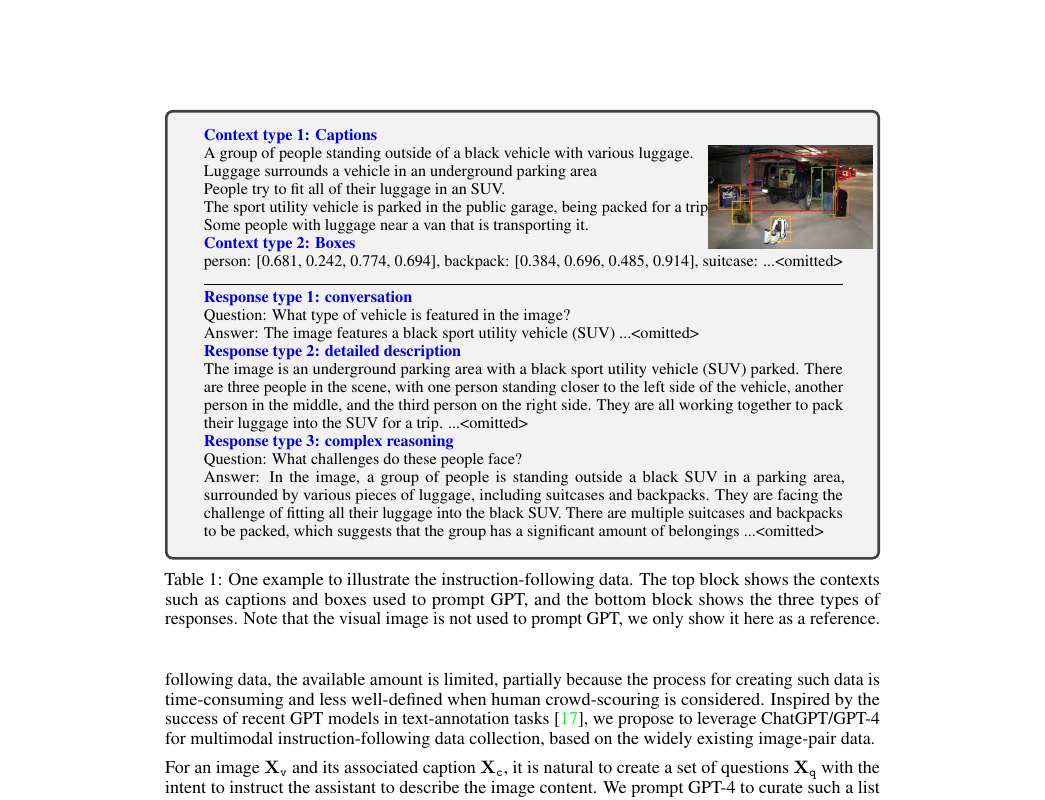
\includegraphics[width=0.98\textwidth]{images/2023-NeurIPS-LLaVA/fig-01.png}
\end{center}

下图表示让GPT4生成Instruction-tuning data的prompt设计\par

\begin{center}
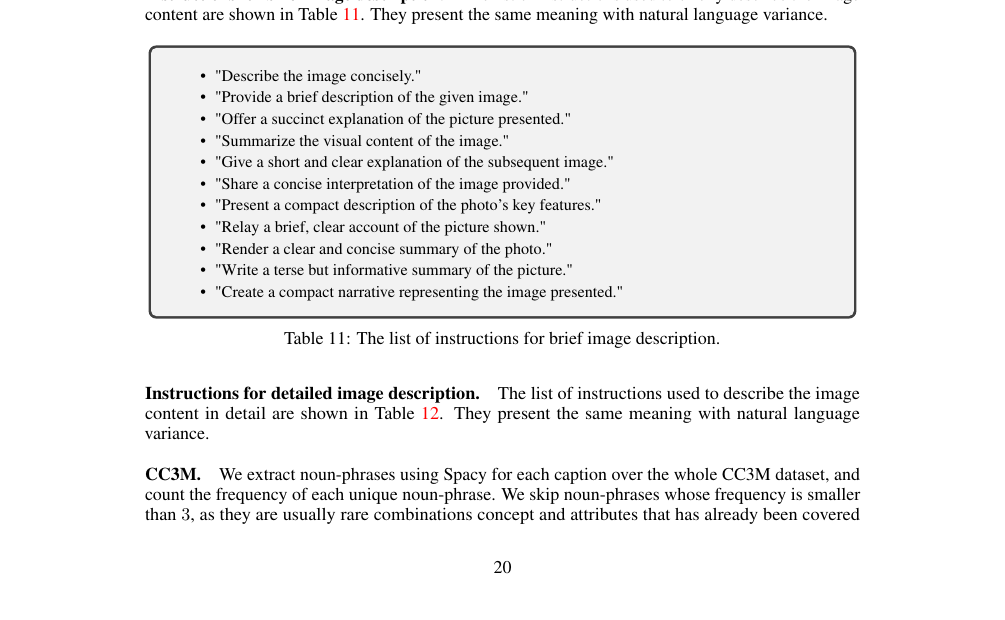
\includegraphics[width=0.98\textwidth]{images/2023-NeurIPS-LLaVA/fig-02.png}
\end{center}

\begin{feishuquote}
在LLaVA的第一个阶段训练（图文对齐预训练）中，还对数据集（CC3M）做了过滤+手动构建Instruction。\par
过滤具体方案是使用Spacy库统计每个唯一的名词短语的频数，删除频数小于3的数据，以及对于频数超过100的，随机选择一个数量为100的子集。（过滤掉出现频率过小的名次）\par
\end{feishuquote}

\begin{feishubox}{callYellow}{🌟}
LLaVA 的 \textbf{指令跟随数据格式} 本质上是 \textbf{用户提出问题或需求（Human）→ 模型生成回答（Assistant）}，具体有：\par
\begin{enumerate}
\item \textbf{对话模式}（提问-回答）
\item \textbf{详细描述}（完整的图片描述）
\item \textbf{复杂推理}（逻辑推理和高级分析）
\end{enumerate}
这种数据格式不仅能训练 LLaVA 进行 \textbf{视觉问答（VQA）}，还能强化它的 \textbf{推理和描述能力}，使其在多模态任务中更具竞争力。\par
\end{feishubox}

\par\vspace{1.15em}\noindent{\zihao{-2}\bfseries 3. 模型结构}\par\vspace{0.28em}

\begin{center}
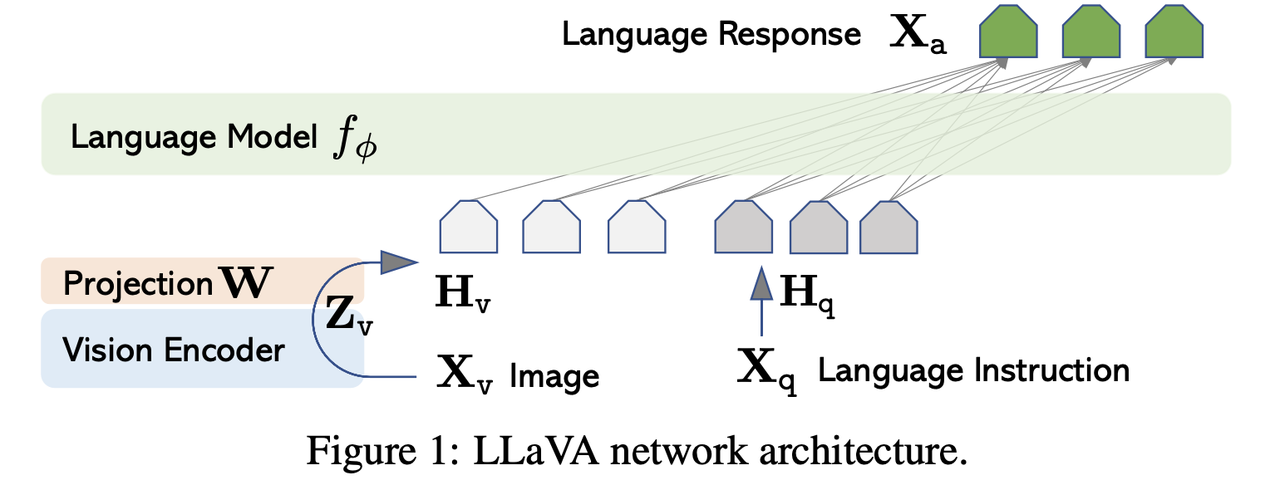
\includegraphics[width=0.98\textwidth]{images/2023-NeurIPS-LLaVA/fig-03.png}
\end{center}

\begin{itemize}
\item \hly{\textcolor{feishuRed}{\textbf{Vision Encoder}}}, CLIP的视觉编码器ViT-L/14, 使用的是倒数第二层的图像特征输出。视觉特征 $Z_v=g(X_v)$
\begin{feishuquote}
这可能是因为 CLIP 的最后一层特征可能比它之前的层更关注全局和抽象的图像属性，而它之前的层可以更关注有助于理解特定图像细节的局部属性\par
\end{feishuquote}
\item \hly{\textcolor{feishuRed}{\textbf{Projection}}}, 线性层Linear，将上面得到的image feature映射到word embedding。实际上是做了一个投影，使用一个可训练的投影矩阵 $W$ 将视觉特征 $Z_v$ 投影到 $H_v$ ，其中 $H_v$ 和文本特征 $H_q$ 在同一特征维度。$H_v=W \cdot Z_v$
\begin{feishuquote}
\textcolor{feishuRed}{Projector使用简单的线性层是比复杂Q-Former是更好的选择}\par
\end{feishuquote}
\item 将已经在同一维度的视觉特征 $H_v$ 和文本特征 $H_q$ 进行concat，然后一起输入到下面的LLM中
\item \hly{\textcolor{feishuRed}{\textbf{Large Language Model}}}, Vicuna 13B（Decoder-Only的LLM，在 \href{https://swfvqxo30ma.feishu.cn/wiki/Y0TEw0IL1iPHNbkFRbBczAy5nUg}{LLaMA系列} 基础上利用对话数据微调得到的），生成Language Response
\end{itemize}

\par\vspace{1.15em}\noindent{\zihao{-2}\bfseries 4. 训练方法}\par\vspace{0.28em}

\begin{feishubox}{callYellow}{🌟}
也是LM Loss + Casual Mask的Decoder范式\par
\end{feishubox}

\textbf{指令跟随数据生成（数据是对话形式）}：对于每个图像 $X_v$ ，生成多轮对话数据 $(X^1_q,X^1_a,\ldots,X^T_q,X^T_a)$ ，其中 $T$ 是总轮数。将它们组织成一个序列，所有答案被视为assistant的响应，第 $t$ 轮的指令 $X^t_{\mathrm{instruct}}$ 为：\par

\bigmath{\mathbf{X}_{\mathrm{instruct}}^{t}=\begin{cases}\text{Randomly choose }[\mathbf{X}_{\mathrm{q}}^{1},\mathbf{X}_{\mathrm{v}}]\text{ or }[\mathbf{X}_{\mathrm{v}},\mathbf{X}_{\mathrm{q}}^{1}], & \text{the first turn }t=1\\ \mathbf{X}_{\mathrm{q}}^{t}, & \text{the remaining turns }t>1\end{cases}}

\textbf{训练目标}：Next token prediction，训练的loss是最大似然概率，即每一步token预测的最大概率乘积，$X_a$ 是答案、$X_v$ 是图像、$X_{\mathrm{instruct}}$ 是指令，$\theta$ 是每个阶段可训练的参数：\par

\bigmath{p(\mathbf{X}_{\mathrm{a}}\mid\mathbf{X}_{\mathrm{v}},\mathbf{X}_{\mathrm{instruct}})=\prod_{i=1}^{L}p_{\theta}(x_{i}\mid\mathbf{X}_{\mathrm{v}},\mathbf{X}_{\mathrm{instruct},<i},\mathbf{X}_{\mathrm{a},<i}),\quad(3)}

模型在训练时只预测assistant应该如何回答和终止的信息，如下图所示，只有答案 $X_a$ 和\incode{<STOP>}的tokens用于计算自回归模型的loss\par

\begin{center}
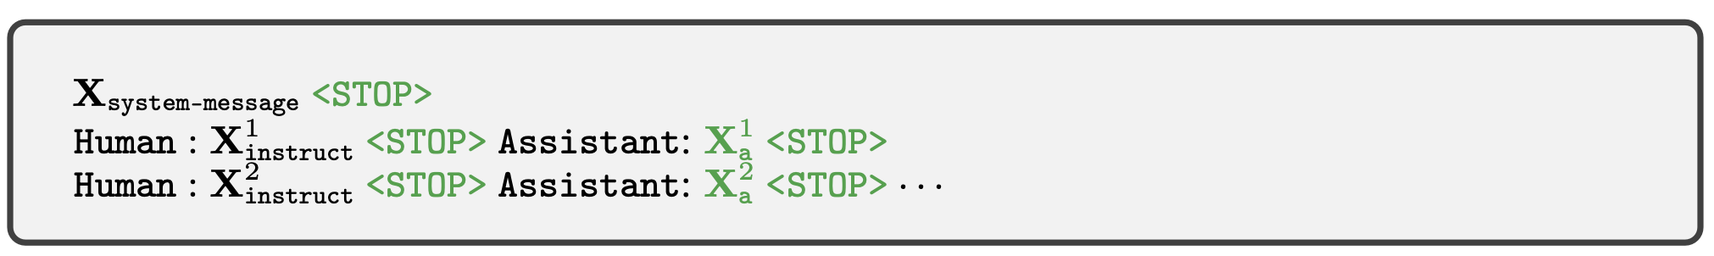
\includegraphics[width=0.98\textwidth]{images/2023-NeurIPS-LLaVA/fig-04.png}
\end{center}

\begin{feishusoft}
\textbf{训练过程分两阶段}：\par
\end{feishusoft}
\begin{enumerate}
\item \textcolor{feishuRed}{\textbf{阶段1 - 图像-文本特征对齐预训练 Pre-training for Feature Alignment}}：\textcolor{feishuBlue}{（冻结的LLM训练一个兼容的visual tokenizer）}
\begin{enumerate}
\item 从CC3M中筛选出595K图像-文本对。这些对通过简单的扩展方法转换为指令跟随数据。
\item 每个样本为\textbf{单轮对话}。
\item 在训练中，\textcolor{feishuRed}{\textbf{仅训练Projector}}用来对齐image-text特征，\textbf{保持视觉编码器和LLM权重冻结}。
\begin{itemize}
\item 真值是图像的原始描述文本。
\item 通过这一步，视觉编码器输出的图像特征可以和预训练的LLM的词向量对齐。
\end{itemize}
\end{enumerate}
\item \textcolor{feishuRed}{\textbf{阶段2 - 端到端指令微调}} \textcolor{feishuRed}{\textbf{Pre-training for Feature Alignment}}：
\begin{enumerate}
\item \textbf{在单轮/多轮对话数据上}\textcolor{feishuRed}{\textbf{微调projection和LLM}}，\textbf{始终保持视觉编码器权重冻结。}使用对话、详细描述和复杂推理数据。
\item 两个具体的任务
\begin{enumerate}
\item 针对日常用户的多模态指令数据\textcolor{feishuBlue}{（让模型更好地理解和回复日常需求）}——\textbf{Multimodal Chatbot 多模态聊天机器人：}在上面构造的158K语言-图像指令跟随数据上进行微调。在conversation、detailed description和complex reasoning三种类型的响应中，conversation\textbf{是多轮交互式的}，而其他两种是单轮交互式的。\textbf{在训练中，每个样本被均匀采样。}
\item 针对科学领域的多模态指令数据\textcolor{feishuBlue}{（加强模型在复杂科学问题上的推理和回答能力）}——\textbf{Science QA 科学问答：}该任务和Multimodal Chatbot差不多，区别在于使用的是公开的数据集ScienceQA benchmark。单轮交互。
\begin{feishuquote}
它的输入除了问题还会有相应的上下文信息，模型的回答需要提供推理过程，以及从多个选择中确定答案\par
\end{feishuquote}
\end{enumerate}
\end{enumerate}
\end{enumerate}

{\renewcommand{\arraystretch}{1.35}%
\begin{tabularx}{\textwidth}{|>{\raggedright\arraybackslash}p{3.2cm}|>{\raggedright\arraybackslash}X|>{\raggedright\arraybackslash}X|>{\raggedright\arraybackslash}X|}
\hline
\cellcolor{tableHead} & \cellcolor{hlOrange}\textbf{Stage 1：特征对齐预训练} & \multicolumn{2}{>{\raggedright\arraybackslash}X|}{\cellcolor{hlYellow}\textbf{Stage 2：指令微调（Visual instruction tuning）}} \\
\hline
\cellcolor{feishuPinkBg}\multirow{2}{*}{目标} & \cellcolor{feishuPinkBg}\multirow{2}{=}{对齐视觉特征和文本特征} & \multicolumn{2}{>{\raggedright\arraybackslash}X|}{\cellcolor{feishuPinkBg}让模型更好地适应视觉问答任务} \\
\cline{3-4}
\cellcolor{feishuPinkBg} & \cellcolor{feishuPinkBg} & \cellcolor{feishuPinkBg}Task 1：Multimodal Chatbot & \cellcolor{feishuPinkBg}Task 2：Science QA \\
\hline
\cellcolor{hlGreen}数据集 & \cellcolor{hlGreen}Filtered from CC3M，595k & \cellcolor{hlGreen}由GPT生成的158K指令跟随数据（对话48K、详细描述23K、复杂推理77K） & \cellcolor{hlGreen}12.7K、4.2K、4.2K \\
\hline
\cellcolor{hlBlue}ViT 是否训练 & \cellcolor{hlBlue}{\feiEmoji{❌}} & \cellcolor{hlBlue}{\feiEmoji{❌}} & \cellcolor{hlBlue}{\feiEmoji{❌}} \\
\hline
\cellcolor{hlBlue}Projection 是否训练 & \cellcolor{hlBlue}{\feiEmoji{✅}} & \cellcolor{hlBlue}{\feiEmoji{✅}} & \cellcolor{hlBlue}{\feiEmoji{✅}} \\
\hline
\cellcolor{hlBlue}LLM 是否训练 & \cellcolor{hlBlue}{\feiEmoji{❌}} & \cellcolor{hlBlue}{\feiEmoji{✅}} & \cellcolor{hlBlue}{\feiEmoji{✅}} \\
\hline
\end{tabularx}}

LLaVA的消融实验：\par
\begin{itemize}
\item 使用CLIP倒数第二层比倒数第一层效果更好
\item CoT作用不大
\item Stage 1的特征对齐预训练很重要，效果提升很大
\item 更大的模型效果更好
\end{itemize}

\begin{center}
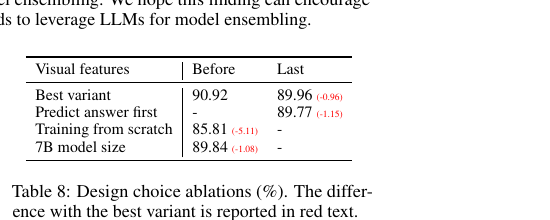
\includegraphics[width=0.86\textwidth]{images/2023-NeurIPS-LLaVA/fig-05.png}
\end{center}

代码的详细解释有一篇blog写的很好，可以去看看：\url{https://zhuanlan.zhihu.com/p/721647840}\par

\par\vspace{1.15em}\noindent{\zihao{-2}\bfseries 5. 总结}\par\vspace{0.28em}

LLaVA 的最大特色在于它力求“\textbf{简单而实用}”。他们没有重复去造一个已经普遍存在或成熟的基础功能，而是把广泛使用的 CLIP VIT-L/14（图像编码器）和基于 Llama 2 的 Vicuna（大语言模型）组合到一起，利用一个\textcolor{feishuRed}{\textbf{轻量的“投影矩阵”}}把图像和文字统一到同一个理解空间，使得LLaVA 在理解和遵守对话环境中的指令方面表现出色，效果优于\textbf{过于复杂}的\href{https://scnajei2ds6y.feishu.cn/wiki/Cb61wEeXDi5NQSkARrbcu8PynEf\#V3VvdDiTuoIVyixgRcNcClO2nhc}{Flamingo的gated cross-attention}、\href{https://scnajei2ds6y.feishu.cn/wiki/AZiVwFmXEirI77kAVzYcOMNVnbh\#NAZtdozkGoFqMQxHJgKc9rCynbe}{BLIP-2的Q-Former}。\par

\end{document}
